% This is "sig-alternate.tex" V1.9 April 2009
% This file should be compiled with V2.4 of "sig-alternate.cls" April 2009
%
% This example file demonstrates the use of the 'sig-alternate.cls'
% V2.4 LaTeX2e document class file. It is for those submitting
% articles to ACM Conference Proceedings WHO DO NOT WISH TO
% STRICTLY ADHERE TO THE SIGS (PUBS-BOARD-ENDORSED) STYLE.
% The 'sig-alternate.cls' file will produce a similar-looking,
% albeit, 'tighter' paper resulting in, invariably, fewer pages.
%
% ----------------------------------------------------------------------------------------------------------------
% This .tex file (and associated .cls V2.4) produces:
%       1) The Permission Statement
%       2) The Conference (location) Info information
%       3) The Copyright Line with ACM data
%       4) NO page numbers
%
% as against the acm_proc_article-sp.cls file which
% DOES NOT produce 1) thru' 3) above.
%
% Using 'sig-alternate.cls' you have control, however, from within
% the source .tex file, over both the CopyrightYear
% (defaulted to 200X) and the ACM Copyright Data
% (defaulted to X-XXXXX-XX-X/XX/XX).
% e.g.
% \CopyrightYear{2007} will cause 2007 to appear in the copyright line.
% \crdata{0-12345-67-8/90/12} will cause 0-12345-67-8/90/12 to appear in the copyright line.
%
% ---------------------------------------------------------------------------------------------------------------
% This .tex source is an example which *does* use
% the .bib file (from which the .bbl file % is produced).
% REMEMBER HOWEVER: After having produced the .bbl file,
% and prior to final submission, you *NEED* to 'insert'
% your .bbl file into your source .tex file so as to provide
% ONE 'self-contained' source file.
%
% ================= IF YOU HAVE QUESTIONS =======================
% Questions regarding the SIGS styles, SIGS policies and
% procedures, Conferences etc. should be sent to
% Adrienne Griscti (griscti@acm.org)
%
% Technical questions _only_ to
% Gerald Murray (murray@hq.acm.org)
% ===============================================================
%
% For tracking purposes - this is V1.9 - April 2009

\documentclass{sig-alternate}
  \pdfpagewidth=8.5truein
  \pdfpageheight=11truein

\usepackage{bookmark}
\usepackage{nth}
\usepackage{cite}
\usepackage{enumerate} 
\usepackage{graphicx}
\usepackage{rotating}
\usepackage{colortbl}
\usepackage{array}
\usepackage{fixltx2e}
\usepackage[latin9]{inputenc} 
\usepackage{listings}
\usepackage{tabularx}
\usepackage{multirow}
\usepackage[table]{xcolor}
\hyphenation{op-tical net-works semi-conduc-tor}
\usepackage{fmtcount}
\usepackage{booktabs,caption,fixltx2e}
\usepackage[flushleft]{threeparttable}


%suporte cite no natbib
\newcommand{\citep}{\cite}

%constantes para tabelas
\newcommand{\minsize}{0.15\textwidth}
%cor da sombra da tabela
\newcommand{\lightgray}{0.95}
%cor da sombra da tabela
\newcommand{\shadow}{0.8}

%nao faz nada, mas mantem espacos e quebras de linha
\newcommand{\nothing}[1]
{
#1
}
%alias para tamanho padrao
\newcommand{\tablesize}[1]
{
\small{#1}
}

%tamanho padrao de figura de uma coluna
\newcommand{\figwidth}{0.48\textwidth}

%formato padrao de figura
\newcommand{\figext}{eps}
%\newcommand{\figext}{pdf}


%encolhe a distancia entre linhas da tabela
 \renewcommand{\arraystretch}{0.55}

\newcommand{\papertitle}{A Systematic Review on Mining Techniques for Crosscutting Concerns}

%\pdfinfo{
%   /Author (Thiago Gottardi and Rafael Serapilha Durelli)
%   /Title  (A Model-Based Approach for Crosscutting Framework Family Reuse)
%   /CreationDate (default)
%   /ModDate (default)
%   /Subject (SBES2012)
%   /Keywords (Model-Driven Engineering; Framework Reuse; Aspect-Oriented Programming; Crosscutting Framework; Empirical Study.)
%}

\newcommand{\sreal}{Primary 
}

\newcommand{\sspare}{Secondary 
}


\begin{document}
%
% --- Author Metadata here ---
\conferenceinfo{SAC'13}{March 18-22, 2013, Coimbra, Portugal.}
\CopyrightYear{2013} % Allows default copyright year (2002) to be over-ridden - IF NEED BE.
\crdata{978-1-4503-1656-9/13/03}  % Allows default copyright data (X-XXXXX-XX-X/XX/XX) to be over-ridden.
% --- End of Author Metadata ---

\title{A Systematic Review on Mining Techniques for Crosscutting Concerns}


%
% You need the command \numberofauthors to handle the 'placement
% and alignment' of the authors beneath the title.
%
% For aesthetic reasons, we recommend 'three authors at a time'
% i.e. three 'name/affiliation blocks' be placed beneath the title.
%
% NOTE: You are NOT restricted in how many 'rows' of
% "name/affiliations" may appear. We just ask that you restrict
% the number of 'columns' to three.
%
% Because of the available 'opening page real-estate'
% we ask you to refrain from putting more than six authors
% (two rows with three columns) beneath the article title.
% More than six makes the first-page appear very cluttered indeed.
%
% Use the \alignauthor commands to handle the names
% and affiliations for an 'aesthetic maximum' of six authors.
% Add names, affiliations, addresses for
% the seventh etc. author(s) as the argument for the
% \additionalauthors command.
% These 'additional authors' will be output/set for you
% without further effort on your part as the last section in
% the body of your article BEFORE References or any Appendices.

\numberofauthors{5} %  in this sample file, there are a *total*
% of EIGHT authors. SIX appear on the 'first-page' (for formatting
% reasons) and the remaining two appear in the \additionalauthors section.
%
\author{
% You can go ahead and credit any number of authors here,
% e.g. one 'row of three' or two rows (consisting of one row of three
% and a second row of one, two or three).
%
% The command \alignauthor (no curly braces needed) should
% precede each author name, affiliation/snail-mail address and
% e-mail address. Additionally, tag each line of
% affiliation/address with \affaddr, and tag the
% e-mail address with \email.
%
% 1st. author
\alignauthor
Rafael S. Durelli\\
       \affaddr{ICMC - USP}\\
       \affaddr{S\~{a}o Carlos, SP, Brazil}\\
       \email{rdurelli@icmc.usp.br}
% 2nd. author
\alignauthor Daniel S. M. Santib\'{a}\~{n}ez\\
       		\affaddr{DC - UFSCar}\\
       		\affaddr{S\~{a}o Carlos, SP, Brazil}\\
       		\email{daniel.santibanez@dc.ufscar.br}
\and
% 3rd. author
\alignauthor 
Nicolas Anquetil\\
       \affaddr{RMoD Team - INRIA}\\
       \affaddr{Lille, France}\\
       \email{Nicolas.Anquetil@inria.fr}
% 4th. author
\alignauthor 
M\'arcio E. Delamaro\\
       \affaddr{ICMC - USP}\\
       \affaddr{S\~{a}o Carlos, SP, Brazil}\\
       \email{delamaro@icmc.usp.br}
% 5th. author
\alignauthor 
Valter Vieira de Camargo\\
       \affaddr{DC - UFSCar}\\
       \affaddr{S\~{a}o Carlos, SP, Brazil}\\
       \email{valter@dc.ufscar.br}
}


\date{30 July 1999}
% Just remember to make sure that the TOTAL number of authors
% is the number that will appear on the first page PLUS the
% number that will appear in the \additionalauthors section.


\maketitle
%abstract

\begin{abstract}
\underline{Background:} The several maintenance tasks a system is submitted during its life usually cause its architecture deviates from the original conceivable design, ending up with scattered and tangled concerns across the software. The research area named concern mining attempts to identify such scattered and tangled concerns to support maintenance and reverse-engineering. \underline{Objectives:} The aim of this paper is threefold: (\textit{i}) identifying techniques employed in this research area, (\textit{ii}) extending a taxonomy available on the literature and (\textit{iii}) recommending an initial combination of some  techniques. \underline{Results:} We selected  62 papers by their mining technique. Among these papers, we identified 18 mining techniques for crosscutting concern. Based on these techniques, we have extended a taxonomy available in the literature, which can be used to position each new technique, and to compare it with the existing ones along relevant dimensions. As consequence, we present some combinations of these techniques taking into account high values of precision and recall that could improve the identification of both Persistence and Observer concerns. The combination that we recommend may serve as a roadmap to potential users of mining techniques for crosscutting concerns.

<<<<<<< HEAD
Ok vamos ver o que esse trem realmente vai funcionar ou não eu não quero nem saber vai funcionar sim

=======
Agora eu vou tentar apreender a colocar um merge que eu quero ver se esse trem realmente funciona como todos nos estamos tentar acreditar em pegadinha de malandro.
>>>>>>> mudarVersaoDOProjeto
\end{abstract}


% A category with the (minimum) three required fields
\category{D.2}{Software Engineering}{Miscellaneus}

\keywords{Systematic Review, Concern Mining, Aspect Mining, Crosscutting Concerns.}

\section{Introduction}
	A possible definition for ``software concern'' is anything which stakeholders regard as a conceptual unit~\cite{Eaddy}. Examples of common software concerns include Persistence, Caching, Synchronization among others~\cite{valterWASP1}. Developers and architects are continuously in need of up-to-date knowledge about the concerns currently implemented in their legacy system, and about the location of these concerns throughout the code. For example, during maintenance and reengineering, when there are bugs to be fixed, the maintenance task affects the whole implementation of a concern, and possibly to other concerns with which the fixed concern interacts.

Mining techniques for crosscutting concerns are indispensable for software maintenance, reverse engineering, reengineering and even for re-documentation~\cite{Marin2007}. However, manually applying a mining technique for crosscutting concern is difficult and error-prone. This came about because, legacy systems tend to: (\textit{i}) have complex architectures with several clones spread out throughout the source code, (\textit{ii}) involve several kinds of crosscutting concerns, e.g., patterns, architectural styles, business rules and non-functional properties and (\textit{iii}) be very large, making the manual mining impractical. Thus, there is a need to use techniques and fully or semi-automated tools, which can aid software engineers to locate crosscutting concern into the legacy systems. In this context, the research area which aims to investigate techniques and tools to improve the mining of crosscutting concerns is known as ``concern mining".

The aim of this paper is threefold. First, we aim to identify techniques employed in the research area herein described. Therefore, we have carried out a systematic review identifying  mining techniques for crosscutting concerns. Second, we intent to extend the taxonomy presented by Kellens et al.~\cite{Kellens}. Thus, we selected 62 papers and among them, we identified 18 mining techniques for crosscutting concerns. This taxonomy was proposed in 2007 and it needs to be updated because we found 7 new techniques developed in the past few years. Third, we recommend possible combinations of these techniques/tools that might improve recall and precision metrics for both Persistence and Observer concerns. We recommend four combinations of techniques discovered herein in order to improve recall and precision for Persistence concern. Similarly, we proposed two initial combinations of techniques identified to make better recall and precision metrics for Observer concern. This combination can be a motivation for potential users to improve the identification of well-known concerns.


%The aim of this paper is to  identify a large amount of techniques related to crosscutting concern mining. Therefore, we have carried out a systematic review identifying  mining techniques for crosscutting concern in the literature. As a consequence, we have discovered that in the last years a considerable number of mining techniques for crosscutting concern are available. Another aim of this paper is to present a roadmap of possibles combinations of the discovered techniques based on the precision and recall metrics. This combination can be a motivation for potential users  to identify remaining open research questions, possible avenues for future research and to decide  which techniques are most suitable to improve the identification of well-known concerns. Another motivation is that previous studies - described in Section~\ref{related} - the authors realized a review without follow a systematic process in the foregoing research area, as consequence, some techniques could be left out in their review. Moreover, the authors devised a comparative framework and taxonomy which allowed one to discriminate among the different techniques, however, a set of new techniques has been developed by combining existing approaches or creating it from the scratch. Thus, we argue that the framework proposed by~\cite{Kellens} must be extended in order to fulfill these new techniques.

% This systematic review shows that there are a lot of interesting and important research topics that could be investigated yet. In addition given the techniques identified we also recommend possible combination of them based on the precision and recall metrics to identify remaining open research questions and possible avenues for future research.

%The main motivation is to identify new opportunities for research on mining techniques for crosscutting concern and to devise a roadmap to potential users of mining techniques for crosscutting concerns, to assist potential users in deciding  which techniques are most suitable to improve the identification of well-known concerns.


%. Therefore, we have carried out a systematic review identifying all the available mining techniques for crosscutting concern in the literature. Thus, by using this review others researches can identify which mining techniques for crosscutting concern exists, which ones is more used and gather information regard which technique accomplish the needs of their projects. Another motivation is that previous studies - described in Section~\ref{related} - the authors realized a review without follow a systematic process in the foregoing research area. Consequently, some techniques could be left out in their review.

This paper is organised as follows: In Section~\ref{method} presents how we have planned, conducted, reported and validated the systematic review. In addition, in this section there is also an extend taxonomy which was firstly proposed by Kellens et al.~\cite{Kellens}. In Section~\ref{threats} there are the threats to validity of our study. Section~\ref{related} presents a related work. Concluding remarks are made in Section~\ref{conclusion}.
	

\section{The Systematic Review}\label{method}
	This study has been undertaken as a systematic review based on the guidelines proposed by Kitchenham and Brereton~\cite{Kitchenham}. According to them, in order to conduct a systematic review, it is advisable to follow three main phases: (\textit{i}) planning the review, (\textit{ii}) conducting the review and (\textit{iii}) reporting the review. Furthermore, in this paper we have used Visual Text Mining (VTM) technique to support the studies selection~\cite{Malheiros:2007}. VTM uses text mining algorithms and methods combined with interactive visualisations. Therefore, it can help the user making sense of a collection of primary studies, without actually reading all of them. In this case the studies were reading partially or full. The following sections present details on how each phase was carried out.

%\begin{figure}[!h]
%\centering
  % Requires \usepackage{graphicx}
%  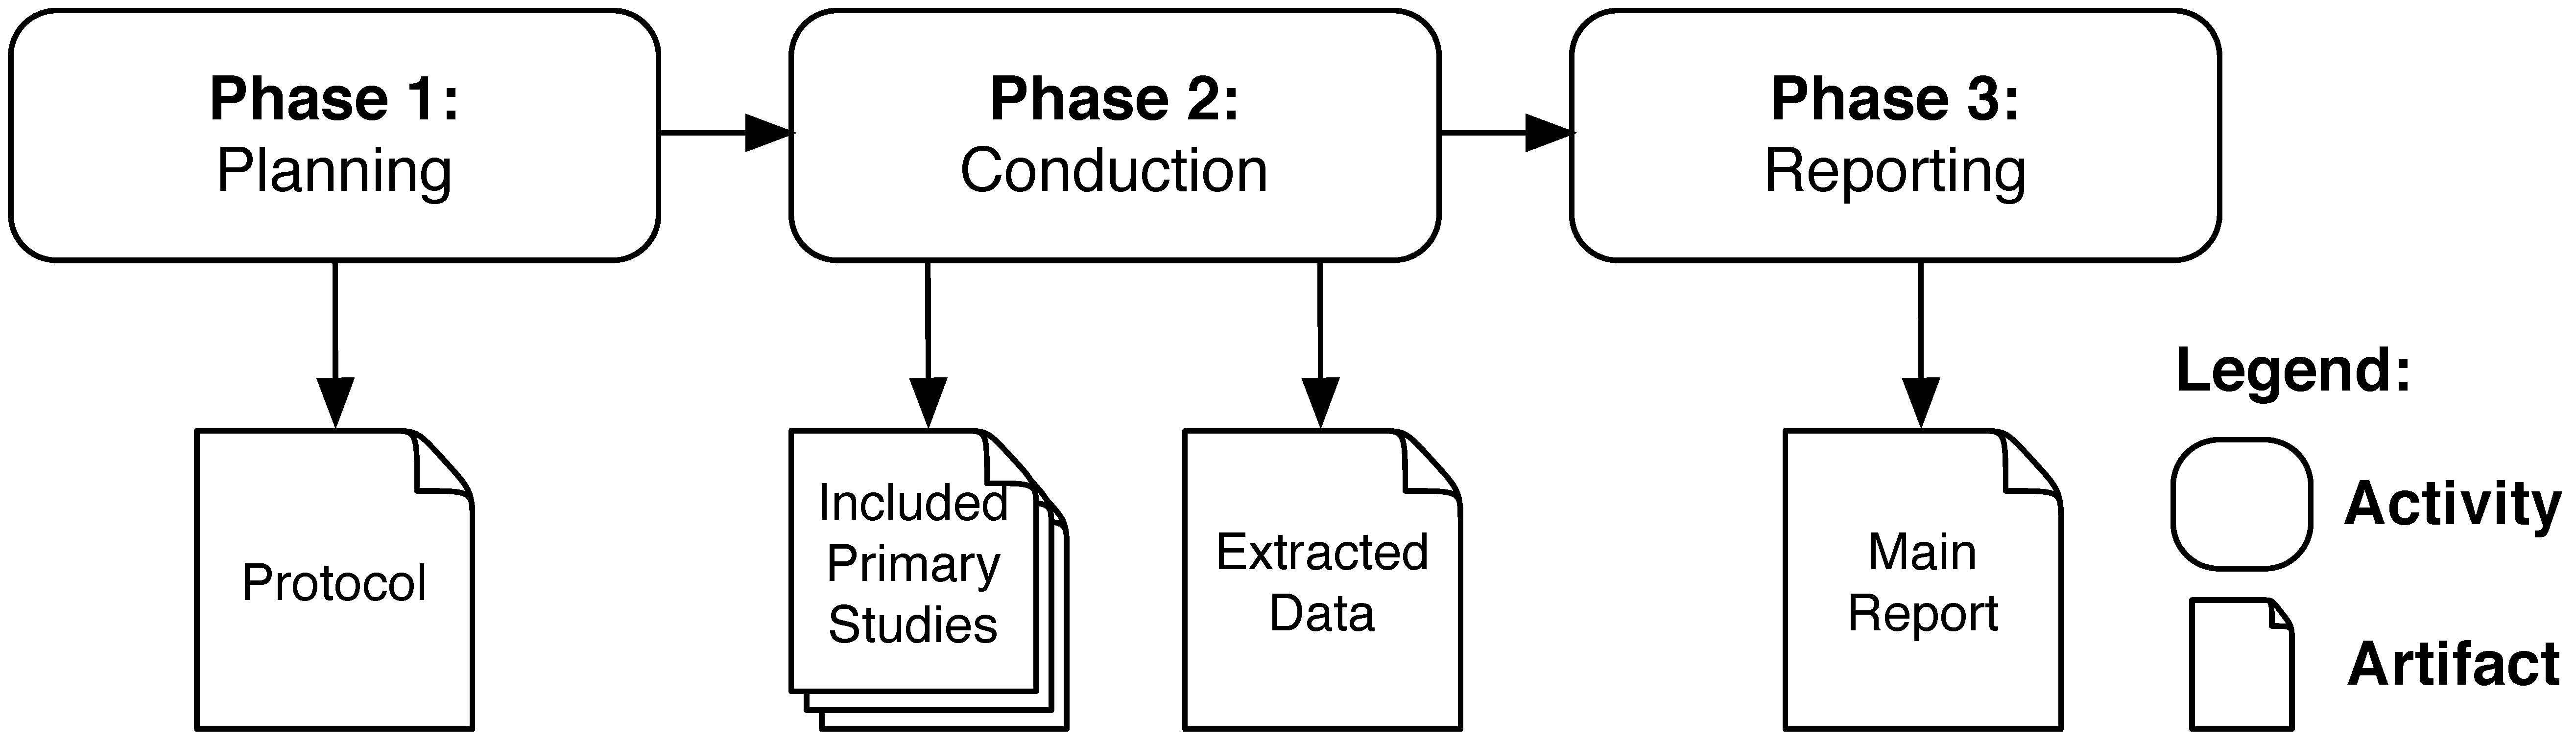
\includegraphics[scale=0.10]{figuras/process}
%\caption{Systematic review process (Adapted from Kitchenham~\cite{Kitchenham}).}
%\label{process_systematic_review}
%\end{figure} 
	\subsection{Planning the Systematic Review\label{planning}}
		In this phase we have defined the review protocol. This protocol contains: (\textit{i}) the research questions, (\textit{ii}) the search strategy, (\textit{iii}) the inclusion and exclusion criteria and (\textit{iv}) the data extraction and synthesis method.

Research questions must embody the review study purpose. Moreover, these questions reflect the general scope of the review study. The scope is comprised of population (i.e., population group observed by the intervention), intervention (i.e., what is going to be observed in the context of the planned review study), and outcomes of relevance (i.e., the results of the intervention). Furthermore, during the conduction of this step, it was also necessary to establish the scope of the review study. According to the systematic review process~\cite{Kitchenham}, the scope has to be established using the PICO criteria. Thus, herein our \textbf{Population} is published scientific literature reporting on some existing mining technique for crosscutting concerns. The \textbf{Intervention} is published scientific literature interested with mining technique for crosscutting concerns. The \textbf{Comparison} is not applied herein. Finally, the \textbf{Outcomes of relevance} is an overview of the studies that have been conducted in the field of crosscutting concern mining, emphasizing primary studies that report on the techniques used in the research area, from observing such an aggregated data set, we also intend to provide insight into the frequencies of publication over time to inspect trends.   

%\begin{itemize}

%\item \textbf{Population:} published scientific literature reporting on some existing mining techniques for crosscutting concern.

%\item \textbf{Intervention:} published scientific literature concerned with mining techniques for crosscutting concern. Furthermore, we also aim at determining which techniques are the most used within academic settings.

%\item \textbf{Comparison:} No applied herein.

%\item \textbf{Outcomes of relevance:} an overview of the studies that have been conducted in the field of crosscutting concern mining, emphasizing primary studies that report on the techniques used in the research area. From observing such an aggregated data set we also intend to provide insight into the frequencies of publication over time to inspect trends.

%\end{itemize} 

As described before, the objective of this review is to find out \textbf{which techniques are employed in mining techniques for crosscutting concerns. Moreover, we intent to extend the the taxonomy presented by Kellens et al.~\cite{Kellens}. Finally, we also want to recommend possible combination of the identified techniques in order to identify remaining open research questions and possible avenues for future research}. In order to achieve such objectives we worked out five research questions. The questions are:

\begin{description}

\item[\textbf{RQ$_1$:}] What are the mining techniques that are currently explored in the literature?

\item[\textbf{RQ$_2$:}]  Which assessment techniques have been employed to evaluate these techniques and what are the results for common concerns?

\item[\textbf{RQ$_3$:}]  Is there any difference in the precision and recall metrics when different techniques are used for mining the same concern?

\item[\textbf{RQ$_4$:}] Given a set of concerns, which are the most indicated techniques for performing the mining?

\item[\textbf{RQ$_5$:}] How can someone combine the techniques for improving the precision and recall metrics?

%\item[\textbf{RQ$_3$:}]  Considering the techniques that we found, which ones have automated support?

\end{description}

Afterwards, we have defined the search string and chosen the electronic databases. The search string was created based upon the following keywords: \textit{approach, method, technique, methodology, aspect oriented, aspect-oriented, aspect mining, concern mining, coding mining, code mining, crosscutting concerns, cross-cutting concerns, Separation of Concern, SoC}. A sophisticated search string was constructed using boolean operators i.e., \textit{AND}, \textit{OR} and \textit{NOT}. Figure~\ref{search_string} shows the search string elaborated. The search have encompassed electronic databases which are deemed as the most relevant scientific sources~\cite{Dyba} and therefore likely to contain important primary studies. We have used the search string on the following electronic databases: \textit{ACM} (portal.acm.org), \textit{IEEE} (ieeexplore.ieee.org), \textit{Scopus} (scopus.com) and \textit{Springer} (springer.com/lncs). %Furthermore, no limits were placed on date of publication with a view to not restrict the review study scope. %Aimed at keeping track of the selected papers, we used JabRef\footnote{http://jabref.sourceforge.net/}, an open source system for bibliography reference management. 

\begin{figure}[!h]
\centering
  % Requires \usepackage{graphicx}
  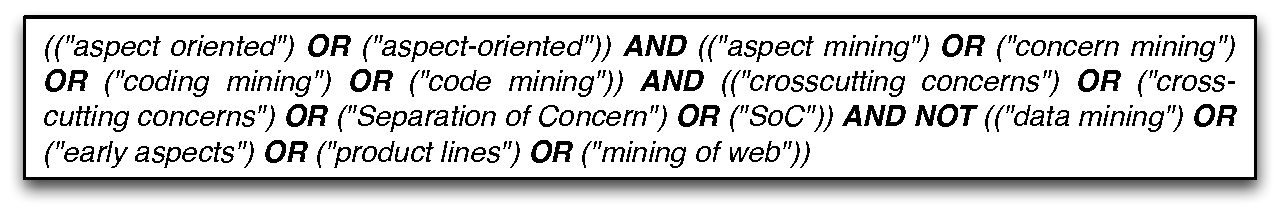
\includegraphics[scale=0.35]{figuras/search_string}
\caption{Search String.}
\label{search_string}
\end{figure} 

Then, in order to determine which primary studies are relevant to answer our research questions, we have applied a set of inclusion and exclusion criteria. Inclusion criteria devised and applied are:

\begin{enumerate}[(a)]%for small alpha-characters within brackets.
\item \textbf{The primary study presents at least one mining technique for crosscutting concern:} the encountered techniques must assist the software engineer in the crosscutting concern mining.
\item \textbf{The primary study presents at least one type of evaluation technique for mining techniques for crosscutting concern:} without the results of the evaluation we neither would be able to make comparisons desired nor would we propose a set of combination of the identified techniques. 
%\textbf{IC$_1$:} the primary study presents at least one mining technique for crosscutting concern
\end{enumerate}

Not all of these criteria must be present for every primary study. However, at least the former (a) must be present. If all criteria were mandatory, the number of selected techniques would decrease significantly.

Exclusion criteria devised and applied are:
\begin{enumerate}[(a)]
\item \textbf{The primary study presents data mining technique. Nevertheless, such technique is applied to databases and not for crosscutting concern mining:} techniques which are applied to databases were not included, since this sort of techniques is outside the scope of this paper.
\item \textbf{The primary study is a short paper:} papers with two pages or less were not considered herein, since we considered that this kind of study do not own sufficient information. 
\end{enumerate}

% \textbf{IC$_1$:} the primary study presents at least one mining technique for crosscutting concern and \textbf{IC$_2$:} the primary study presents at least one type of evaluation technique for crosscutting concern. And the following exclusion criteria: \textbf{EC$_1$:} the primary study presents data mining technique, however, such technique is applied to databases and not for crosscutting concern mining and \textbf{EC$_2$:} the primary study is a short paper (papers with twos pages or less).

%\begin{description}

%\item[\textbf{IC$_1$:}] The primary study presents at least one mining technique for crosscutting concern

%\item[\textbf{IC$_2$:}] The primary study presents at least one type of evaluation technique for crosscutting concern.

%\end{description}

%and the following exclusion criteria:

%\begin{description}

%\item[\textbf{EC$_1$:}] The primary study is not about mining techniques for crosscutting concern.

%\item[\textbf{EC$_2$:}] The primary study presents data mining technique. However, such technique is applied to databases and not for crosscutting concern mining.

%\item[\textbf{EC$_3$:}] The primary study is not available in an electronic format.

%\item[\textbf{EC$_3$:}] The primary study is a short paper (papers with twos pages or less).

%\item[\textbf{EC$_5$:}] The primary study is written neither english nor portuguese.

%\end{description}

We devised data extraction forms to accurately record the information obtained by the researchers from the primary studies. The form for data extraction provides some standard information, such as (\textit{i}) name of the techniques identified, (\textit{ii}) date of data extraction, (\textit{iii}) title, authors, journal, publication details and (\textit{iv}) a list of each conclusion and statement encountered for each sub-question. 

During the extraction process, the data of each primary study were independently gathered by two reviewers. The review was performed in August, 2012 by a M.Sc. and a Ph.D. students; the achieved results were crossed and then validated. All the results of the search process are documented in the web material\footnote{http://tinyurl.com/99spmaz}. Therefore, it is clear to others how thorough the search was, and how they can find the same documents.

	\subsection{Conducting the Systematic Review\label{conducting}}
		%In Figure 2~\ref{process} the three steps of the conduction phase. As can be seen, in Step 1, we identified primary studies in the digital libraries. The digital libraries Scopus has returned more primary studies than the others(262), i.e., IEEE, ACM and Springer have returned 215, 202 and 127, respectively. Possibly, this came about because this digital library indexes studies of others libraries, such as IEEE and Springer. Summing up, we have gotten 802 primary studies in the Step 1. In the Step 2 we have selected the primary studies by means of reading the titles and abstracts and the application of the inclusion and exclusion criteria. As a result, we have gotten a total of 124 primary studies that were read entirely, so the upshot obtained in the Step 3 were 62. Among these 62 primary studies we have identified 18 mining techniques for crosscutting concern. Therefore, each included primary study was assigned to one or more techniques.
%
%\begin{figure}[!h]
%\centering
%  % Requires \usepackage{graphicx}
%  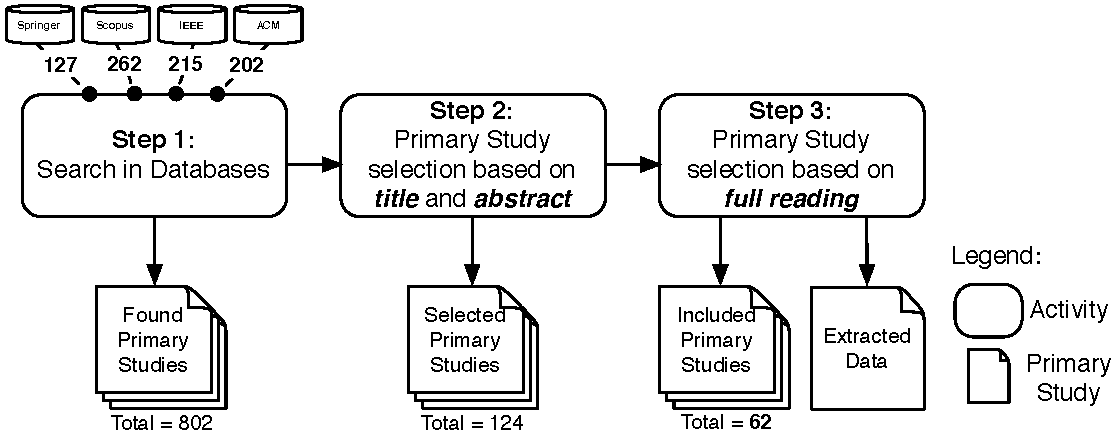
\includegraphics[scale=0.4]{figuras/process_conducted}
%\caption{Papers retrieved from each electronic database, total of candidate studies and the final set.}
%\label{process}
%\end{figure} 

In this phase, firstly we identified primary studies in the digital libraries. The digital libraries Scopus has returned more primary studies than the others (262), i.e., IEEE, ACM and Springer have returned 215, 202 and 127, respectively. Possibly, this came about because this digital library indexes studies of others libraries, such as IEEE and Springer. Summing up, we have gotten 802 primary studies. Afterwards we have selected the primary studies by means of reading the titles and abstracts and the application of the inclusion and exclusion criteria. As a result, we have gotten a total of 124 primary studies that were read entirely, so the upshot obtained were 62 studies. 

Among these 62 primary studies we have identified 18 mining techniques for crosscutting concern. Therefore, each included primary study was assigned to one or more techniques. In the following we outline each of the techniques: 

\begin{itemize}

\item \textit{Execution Patterns (EP)}: During program execution, program traces are generated, which reflect the run-time behavior of a software system. These traces are then investigated for recurring execution patterns. In~\cite{Breu:2004:AMU:1025115.1025235} the authors introduce the notion of execution relations between method invocation. In other words, the basic idea of EP is to observer run-time behavior of software system and to extract information from the execution of the programs. As example, consider the Figure X, wherein that capitals represent methods names. According to Breu and Krinke~\cite{Breu:2004:AMU:1025115.1025235} exist four different execution relations, they are: (\textit{i}) outside-before, see Figure X, where B is called before A, (\textit{ii}) outside-after, where A is called after B, see Figure X, (\textit{iii}) inside-first, G is the first call in C and (\textit{iv}) inside-last, H is the last call in C. 


%This technique analyses program traces reflecting the run-time behavior of a system in search of recurring execution patterns. Thus, their mining algorithm discovers concern candidates based on recurring patterns of method invocations~\cite{Breu:2004:AMU:1025115.1025235}.

\item \textit{Dynamic Analysis (DA)}: DA is the analysis of the properties of a running program, whereas to static analysis, which examines a program's text to derive properties that hold for all executions, DA derives properties that hold for one or more executions by examination of the running program. 
While DA cannot prove that a program satisfies a particular property, it can detect violation of properties as well as provide useful information to programmers about the behavior of their programs. 
The usefulness of DA supplies from two of its essential characteristic:
\begin{itemize}

\item Precision of information: DA typically involves instrumenting a program to examine or record certain aspects of its run-time state. This instrumentation can be tuned to collect precisely the information needed to address a particular problem. For example, to analyze the shape of data structures created by a program (lists, trees, dags, etc.), an instrumentation tool can be created to record the linkages among heap-allocated storage cells;

\item Dependence on program inputs: the very thing makes DA incomplete also supplies a powerful mechanism for relating program inputs and outputs to program behavior. With DA it is straightforward to relate changes in program inputs to changes in internal program behavior and program outputs, since all are directly observable and linked by the program execution. Viewed in this light, dynamic and static analysis might be better termed ``input-centric'' and ``program-centric'' analysis, respectively.
 

\end{itemize}

Dynamic and static analyses are complementary techniques in a number of dimensions, them are: 

\begin{itemize}

\item Completeness: In general, dynamic analyses generate ``dynamic program invariants'', properties which are true for the observed set of execution. Static analysis can help determine or not these dynamic ``invariants'' truly are invariants over all program executions. In the cases where the dynamic and static analyses disagree, there are two possibilities: (\textit{i}) the dynamic analysis is in error because it did not cover a sufficient number of executions, (\textit{ii}) the static analysis is in error because it analyzed infeasible path;

\item Scope: Because dynamic analysis examines one very long program path, it has the potential to discover semantic dependencies between program entities widely separated in the path. Static analysis typically is restricted in the scope of a program it can analyze and efficiently, and may have troubles discovering such ``dependencies at a distance''.

\item Precision:  DA has the benefit of examining the concrete domain of the program execution. In other hands, static analysis must abstract over this domain in order to ensure termination of the analysis, thus, it can lose information. 

\end{itemize}

%DA deals with task scenarios that formulate the user-system interactions in an informal or semi-formal manner. 
%DA with its suitability in extraction system functionality has several challenges compared to the Static Analysis (SA): 
%(\textit{i}) a SA usually generates a complete set of software facts through parsing or lexical analysis of the source code based on a domain model, 
%whereas in DA only a small subset of the possible dynamic traces are extracted, 
%(\textit{ii}) obtaining meaningful knowledge from the extracted execution traces is a difficult task that affects the applicability of the DA, 
%(\textit{iii}) the large sizes of the execution traces that are caused by program constructs such as loops and recursions may disfunction the whole dynamic analysis. 
In the context of discovering possible concerns DA applies FCA\footnote{FCA is a mathematical theory of data analysis which describe relationship between a particular set of objects and a particular set of attributes~\cite{PrissFCA}} to get execution traces.
In other words, the obtained execution traces are analyzed using FCA for identifying methods and classes.  
%In order to discover possible concerns DA applies formal concept analysis (FCA) to get execution traces. 
%A version of the system is executed on a number of use cases. 
%The obtained execution traces are analyzed using FCA for identifying methods and classes. 
Thus, methods belonging to more than one class may indicate presence of scattering code. 
If different methods from same class are specific to more than one use-case may indicate presence of tangling code~\cite{Ceccato:2008:ASM:1545010.1545380}.

\item \textit{Identifier Analysis (IA)}: This technique performs an identifier analysis using FCA algorithm. The assumption behind this approach is that relevant concerns in the source code are reflected by the use of naming conventions in the classes and methods of the system. As input to FCA algorithm, the classes and methods are used as objects and substrings generated from the classes and methods names are used as attributes. The resulting concepts consists out of maximal groups of classes and methods which share a maximal number of substrings~\cite{Tourwe:2004:MAV:1018444.1022149}.

\item \textit{Language Clues (LC)}: The approach uses natural language processing for mining crosscutting concern. The input is a collection of words from the source code and the output, chains of words which are semantically strongly related calculated with an algorithm. In order to mine for crosscutting concerns, they apply the chaining algorithm to the comments, method names, field names and class names of the system. A manual inspection to the resulting chains is needed in order to select possible concerns~\cite{Shepherd:2005:ULC:1083125.1083129}.

\item \textit{Method Clustering (MC)}: This technique starts by putting each method in a separate cluster and then, recursively, merges clusters by similarities in method names~\cite{Bernardi2009CTI}. 

\item \textit{Call Clustering (CC)}: This technique starts from the assumption that if the same methods are called frequently from within different modules, then, they are closely related and must be clustered~\cite{Danfeng}.


\item \textit{Fan-In analysis (FI)}: It is an approach that involves looking for methods that are called from many different call sites and whose functionality is needed across different methods, potentially spread over many classes and packages. 
FI is a semi-automated process consisting of three steps. Firstly, the method with the highest fan-in values need to be identified. Secondly, one have to filter out methods that may have a high fan-in but for which it is unlikely that there is a systematic pattern in their usage that could be exploited in an aspect solution. Common examples are getters and setters, and utility methods as well. Thirdly, the call sites of the high fan-in methods need to be inspected to determine if the method in questions does indeed implement crosscutting functionality. The last step is the most labor intensive, and it is based on an analysis of recurring patterns in, for example, the call sites of the high fan-in method~\cite{Marin:2007:ICC:1314493.1314496}.
%Through fan-in metric, this approach can measure the number of methods that call some other methods.
High fan-in metric values may indicate presence of a crosscutting concern~\cite{Danfeng}.

\item \textit{AST-Based Clone Detection (ACD)}: This technique takes the Abstract Syntax Tree (AST) of the source code into account. The output is a number of clone classes, i.e. groups of code fragments which are considered to be clones of each other~\cite{Bruntink2005}.

\item \textit{Token-Based Clone Detection (TCD)}: This technique is based on lexical analysis of the source code. The output is a number of clone classes, i.e., groups of code fragments which are considered to be clones of each other~\cite{Bruntink2005}.

\item \textit{History Based (HB)}: This technique intends to discover crosscutting concerns by analyzing the changes made in the source code along the time by using software repositories like revision control systems, files and databases~\cite{Mulder:2010:ICC:1862372.1862381}.

\item \textit{Information Retrieval (IR)}: This technique tries to identify concerns. It is based on the similarity between terms used in the concern descriptions and in the program elements, e.g., element names, variable names. The results are ranked and a manual inspection is performed~\cite{Eaddy:2008:CTR:1437898.1438590}.

\item \textit{Parser-Based (PB)}: This technique performs a lexical or syntactic analysis of the source code to locate crosscutting concerns. It is based on the premise that code fragments which share concerns are likely to refer to readily identifiable shared entities such as identifiers and libraries~\cite{Griswold}.

\item \textit{PrefixSpan (PS)}: It is a data mining technique used to identify coding patterns in source code. Each method in a program is translated to a sequence that comprises method call elements and control elements. The algorithm searches for repetitive subsequences that could form a pattern~\cite{Ishio:2008:MCP:1447565.1448040}.

\item \textit{Concern-Peers (CP)}: This technique identifies certain groups of code units that potentially share some crosscutting concerns. These code units, called concern peers, are detected based on their similar interactions (similar calling relations in similar contexts, either internally or externally). The algorithm scan for candidates, i.e., methods with similar code and names, then scan for peers and rank it to recommend possible concerns~\cite{Nguyen2011}. 

\item \textit{Method Call Tree (MCT)}: It uses method call tree to generate method call traces. These traces are then investigated for recurring method patterns based on different constraints, such as, the requirement that the patterns exist in always the same composition and in different calling contexts in the method call trace~\cite{Qu:2007:AMU:1262690.1262897}.

\item \textit{Data-Flow Concern Identification (DF)}: It is a semiautomated approach for concern identification specifically designed to support software understanding. It starts from a set of related variables and uses static dataflow information to determine the concern skeleton, a data-oriented abstraction of a concern~\cite{Trifu:2008:UDI:1545010.1545363}.

\item \textit{Random Walks (RW)}: A random walk is a mathematical formalization of a trajectory that consists of taking successive random steps. This technique performs a random walks on the coupling graphs extracted from the program sources. The algorithm reflects the degrees of ``popularity and significance" for each of the program elements on the coupling graphs. Filtering techniques, exploiting both types of ranks, are applied to produce a final list of candidate crosscutting concerns~\cite{CharlesZhang2011}.

\item \textit{Model-Driven (MD)}: This technique is a model driven approach for concern mining and their separation, which automatically identifies desirable candidate concerns, without requiring input from the user. The concern miner acts as a model transformer converting the source code to a concern-oriented model~\cite{Nora}.

\end{itemize}

The taxonomy proposed by Kellens et al.~\cite{Kellens}, takes into account 3 dimensions: \textit{(i)} static or dynamic analysis; if the technique does a static analysis of the code or dynamic information which is obtained by executing the program or both. \textit{(ii)} Token-Based or structural/behavioral analysis; lexical analysis like sequences of characters, regular expression or abstract syntax trees, type information, message sends, etc. \textit{(iii)} Granularity: The level of granularity of the technique, method level or more fine-grained. 

In this context, we have extended the taxonomy proposed by Kellens et al.~\cite{Kellens} by means of adding the new identified mining techniques. In Figure~\ref{taxonomy}, it is depicted our extended taxonomy. The small rectangles in the middle of the figure represent all of the techniques: the previous ones, proposed by Kellens et al.~\cite{Kellens} and the new ones proposed by us, marked with an asterisk in Figure~\ref{taxonomy}. More specifically, from the 18 techniques identified herein, 7 of them are new and were added to the taxonomy. The new techniques are: PrefixSpan, Information Retrieval, Dataflow, Model-Driven, Random Walks, History-Based, Concern Peers. The details on each of the identified new techniques and algorithms are outside the scope of this paper. Also, the fact of adding new techniques asked for the inclusion of new algorithms in the taxonomy as well. So, we added four algorithms, they are: Vector Space Indexing, Frecuent Itemset, Concern Model, Peer Detection. 
Finally, a new granularity level was added because the history-based technique can search for crosscutting concerns into source code repositories. 

%We argue that this taxonomy could serve as an initial roadmap for crosscutting concern researchers. Moreover, it is could be relevant for tool developers who might have knowledge about the best aspect indicators to use or who may have certain demands about the granularity of the results.



 %This taxonomy could serve as an initial roadmap to crosscutting concern miners and researchers. Each of the 18 mining techniques for crosscutting concern identified are represented by a small rectangle. The six larger rectangles distinguish  `static' from `dynamic' techniques, and `method-level' techniques from techniques which report both `method fragment' and `file-level' as seeds. Finally, the two rounded rectangles on the left partition represent techniques which use `token-based' and `structural/behavioral' ones.

\begin{figure}
\centering
  % Requires \usepackage{graphicx}
  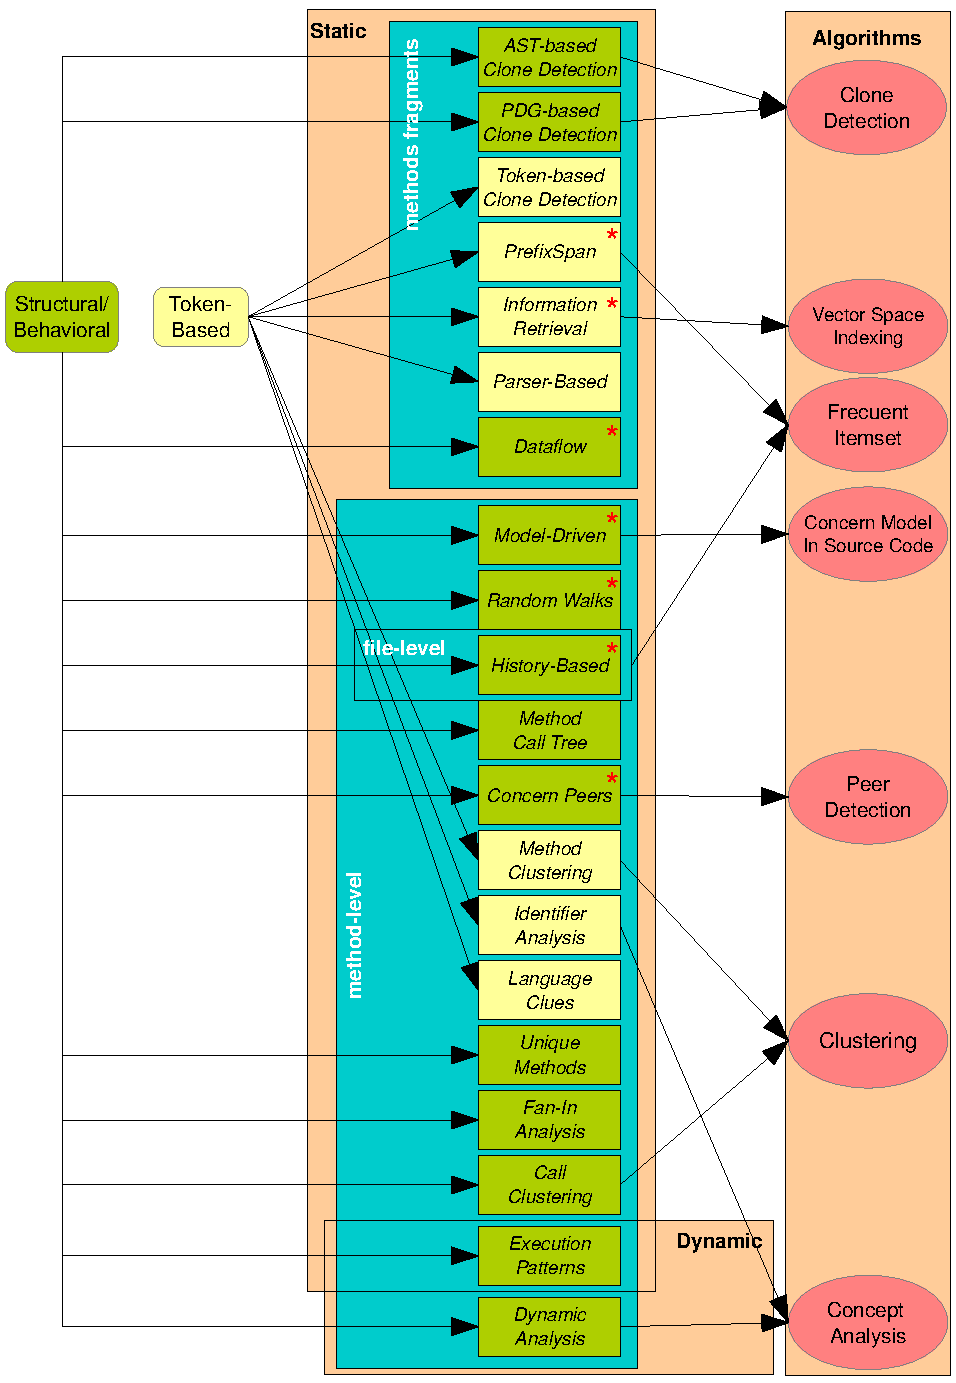
\includegraphics[width=8cm, height=13cm]{figuras/taxonomy}
\caption{The Extended Taxonomy (Adapted from \textit{Kellens et al.}~\cite{Kellens}).}
\label{taxonomy}
\end{figure} 
	\subsection{Validation\label{validation}}
		In validation phase an approach that uses VTM technique and the associated tool - Projection Explorer (PEx) - were applied to support the inclusion and exclusion decisions~\cite{Malheiros:2007}. %PEx adopts a two-dimensional visual representation, known as document map, where each document is mapped to a graphical element on the plane, usually a circle (point), with points relative positions reflecting similarity relationships between the contents of the documents they represent. Thereby, on the layout, similar documents are put close to one another, while dissimilar ones are supposed to be positioned far apart.

\begin{figure}[!h]
\centering
  % Requires \usepackage{graphicx}
 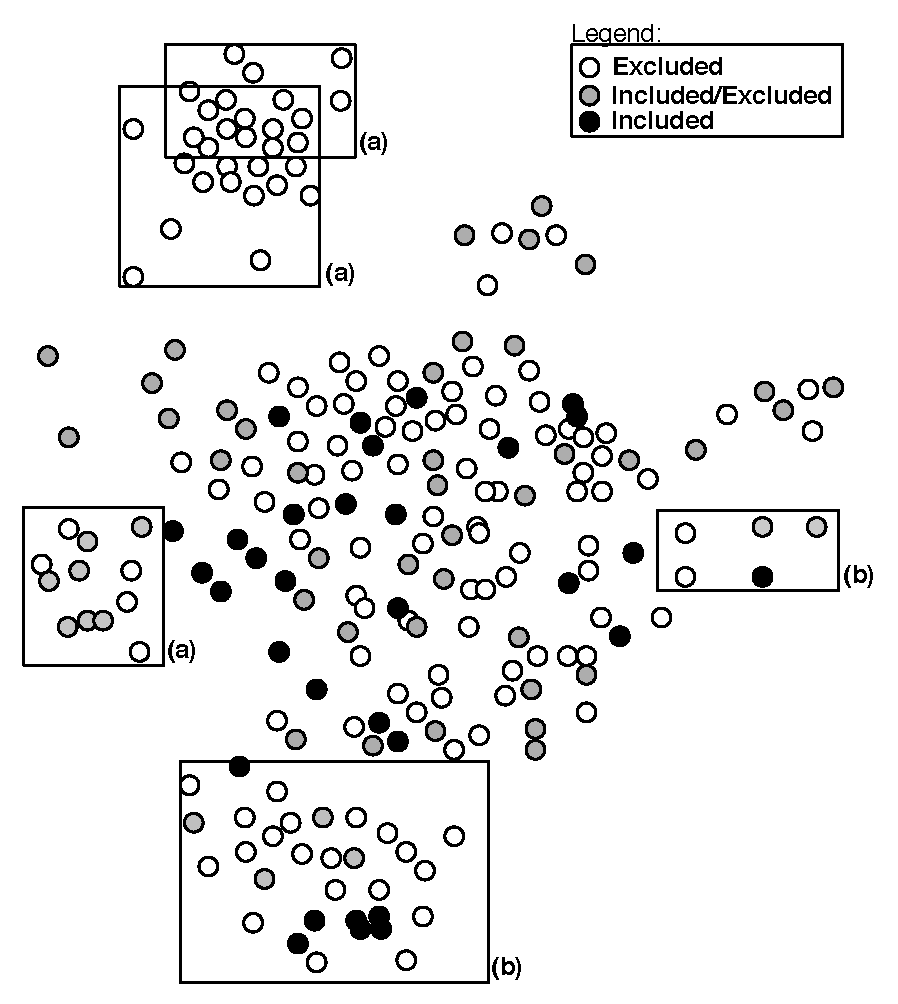
\includegraphics[scale=0.40]{figuras/validation2}
\caption{Document map colored with the history of the inclusions and exclusions of the studies.}
\label{fig:validation}
\end{figure} 

Figure~\ref{fig:validation} presents a document map generated using PEx. This map is composed of 802 primary studies analysed in this review, highlighting them using different shades of gray to differentiate in which of the stages a study was removed from the review. White points are studies excluded in first stage, gray points are the studies excluded in second stage and the black points are the included. The exploration of a document map is conducted in two steps: (\textit{i}) firstly, a clustering algorithm is applied to the document map, creating groups of highly related documents; (\textit{ii}) secondly, the resulting clusters are analysed in terms of:~\textbf{Pure Clusters} - all documents belonging to a cluster have the same classification (all included or excluded, regardless of exclusion stage). Normally, in this case do not need to be reviewed; and~\textbf{Mixed Clusters} - which represent documents with different classification on the same cluster. These cases are hints to the reviewer, and the estuaries grouped should be reviewed following the traditional method. To facility the visualisation, in Figure~\ref{fig:validation} just five clusters generated by PEx are depicted. Examples of pure clusters (all excluded) are identified in Figure~\ref{fig:validation} using label ``(a)'' and therefore do not needed to be reviewed. Mixed clusters (clusters containing black (included) and white or gray (excluded) studies) are identified using label ``(b)'' and they were reviewed by the authors of this paper. At the end, we kept the initial classifications conducted manually, but this technique contributed to a review of studies that could have been wrongly excluded or included previously.  

	
	\subsection{Reporting the Systematic Review\label{reporting}}
		The focus of this section is to present the broad overview of research within crosscutting concern mining we have acquired after classifying and categorizing primary studies. Moreover, we have used information drawn from this overview to answer this review study's research questions.

Aiming to show the frequencies of publication of all identified techniques for mining techniques for crosscutting concerns mining we have plotted a bubble plot, which is depicted in Figure~\ref{map}. Bubble plots are essentially two x-y scatter plots with bubbles in category intersections. The size of each bubble is determined by the number of primary studies that have been classified as belonging to the categories corresponding to the bubble coordinates. This visual summary provides a bird's-eye view that enables one to pinpoint which categories have been emphasized in past research along with gaps and opportunities for future research. 

In Figure~\ref{map} the facets we have used for organizing the map are the crosscutting concern mining techniques and year of publication. Based in this figure it is evident from observing it that we have found out 18 mining techniques for crosscutting concerns, as result we have answered the first part of the RQ$_1$. Based upon this bubble plot, we argue that the answer to second part of the RQ$_1$ is that Fan-In Analysis, Identifier Analysis and Dynamic Analysis are the techniques most used and Program Analysis Based, XScan-Concern-Peers, Data-Flow and Model Driven are the least used. More precisely, among the 62 primary studies included herein, 27 describe Fan-In Analysis, Identifier Analysis or Dynamic Analysis, respectively. In other hands, the techniques with less studies available in literature are Program Analysis Based, XScan-Concern-Peers, Data-Flow and Model Driven. Furthermore, it is argued that Fan-In Analysis, Identifier Analysis and Dynamic Analysis are evidence clusters (i.e., where there may be scope for more complete literature reviews to be undertaken). In contrast, Program Analysis Based, XScan-Concern-Peers, Data-Flow and Model Driven can be deemed as ``evidence desert'' (i.e., wherein better or new research is required). 

%According to this figure, a year-wise distribution of the CD, FI and DA reveals an increase in publication over time, most notable from 2006 to 2008. Moreover, Figure~\ref{frequencies_chart} depicts that the number of publication of these techniques have been stabilized in 2009 to 2011.

\begin{figure*}
\centering
  % Requires \usepackage{graphicx}
  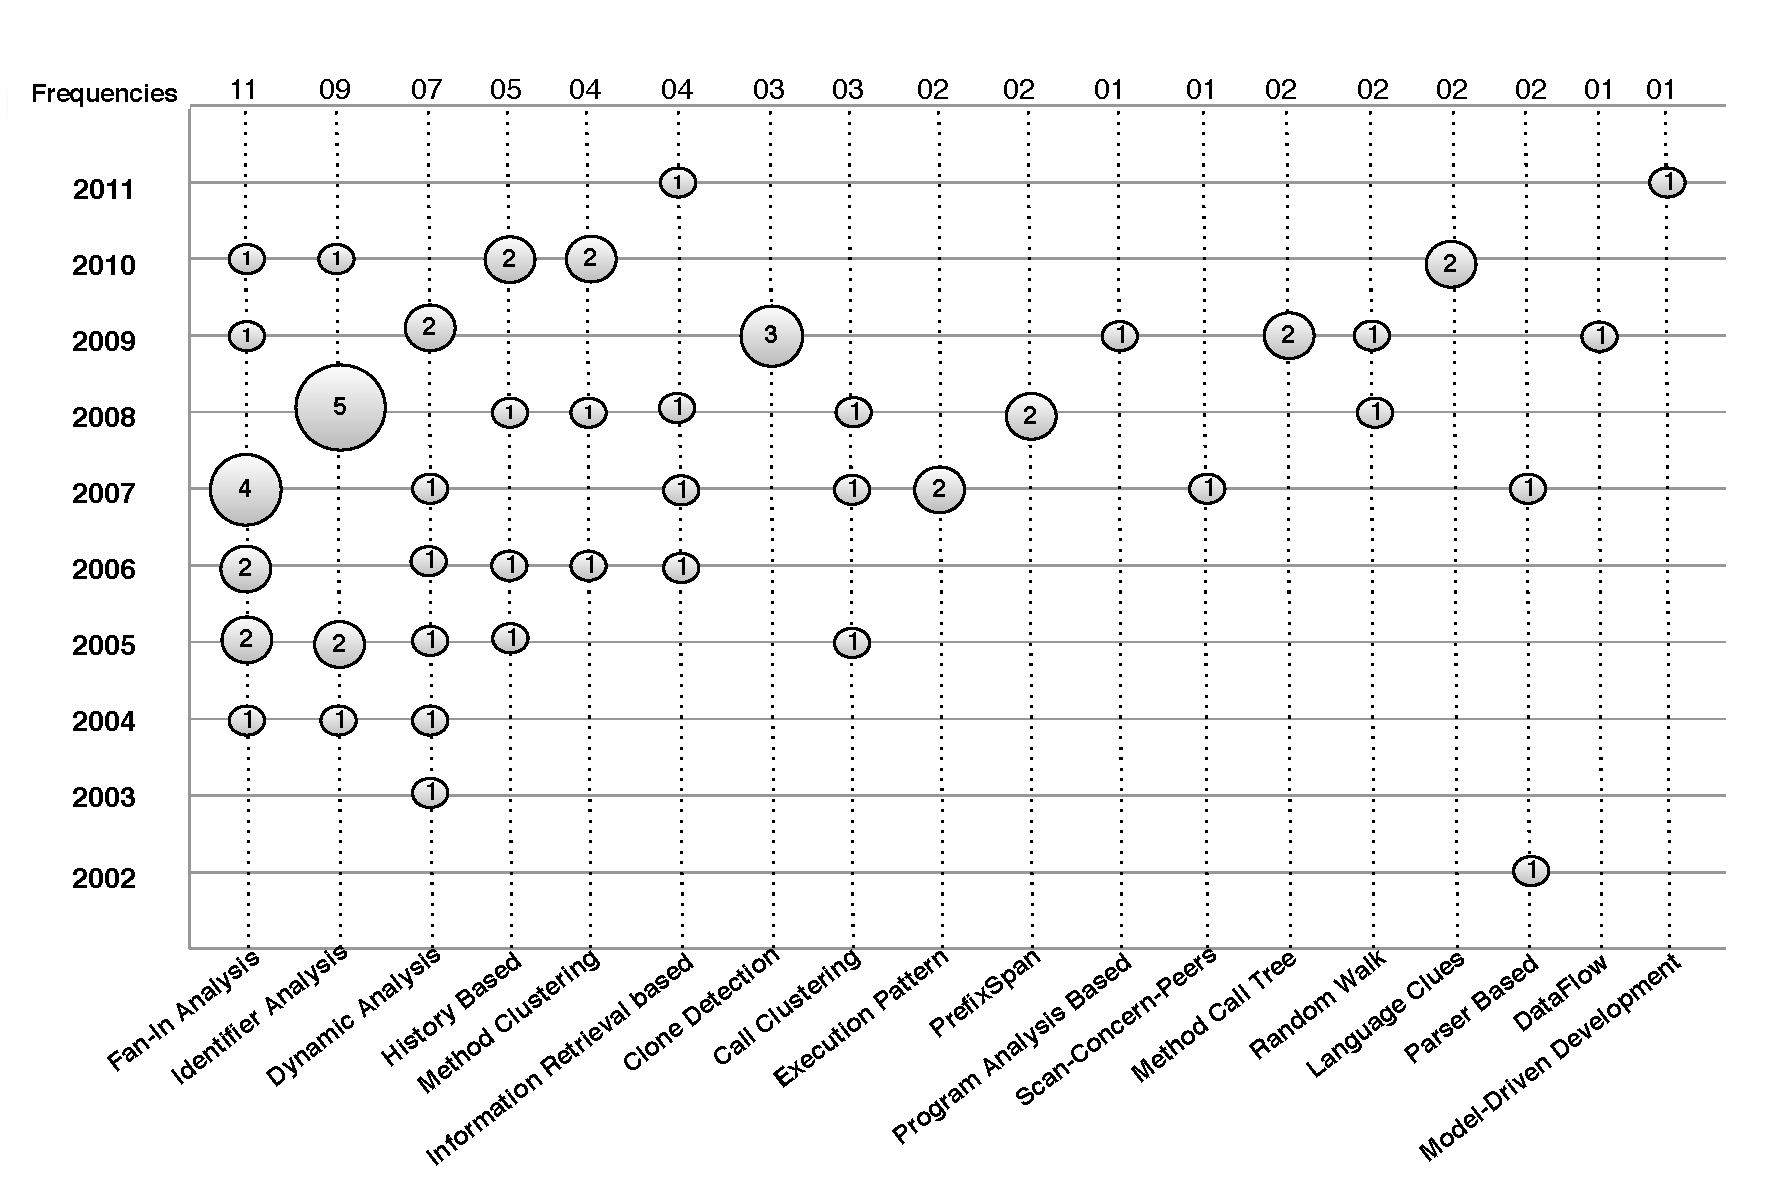
\includegraphics[width=14.5cm, height=7.3cm]{figuras/MapaDasTecnicas}
\caption{Map containing a year-wise distribution of publications on the all techniques found.}
\label{map}
\end{figure*} 

The majority of selected primary studies are published by IEEE, i.e., 20 primary studies. The others primary studies have been selected from ACM, Scopus and Springer, 18, 16 and 8, respectively. As for the publication types, we have selected primaries studies that have been published in conferences, workshops and journals. The majority of the primary studies are conference paper (37), followed by workshop (16) and journal (9).

%\begin{figure}[!h]
%\centering
  % Requires \usepackage{graphicx}
  %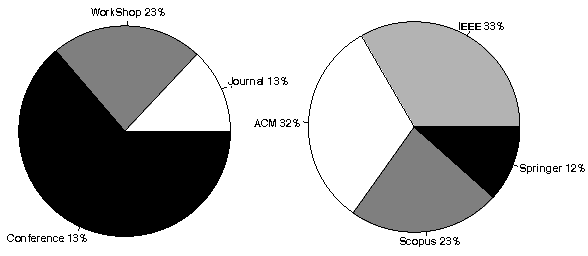
\includegraphics[scale=0.90]{figuras/PublicationTypeAndJounal2}
%\caption{Distribution of primary studies by publication type and distribution of primary studies by electronic database.}
%\label{publication_pie}
%\end{figure} 

\begin{figure}[!h]
\centering
  % Requires \usepackage{graphicx}
  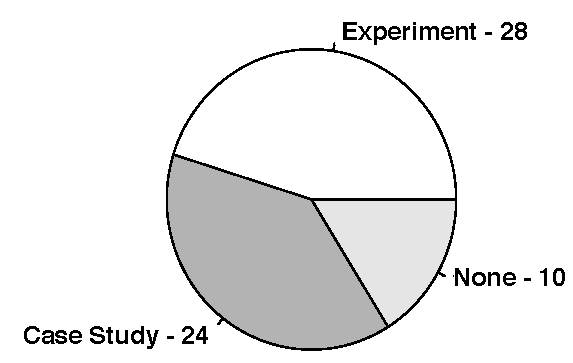
\includegraphics[scale=0.54]{figuras/pieChart}
\caption{Which empirical strategies have been employed.}
\label{empirical_strategies}
\end{figure} 


The way in which a technique is evaluated provides researchers and practitioners with useful information on the approach's quality, effectiveness, robustness, and practical applicability. Evaluating crosscutting concern mining techniques is difficult because defining the program elements that are relevant to a concern may be subjective. Despite this difficulty, researchers have devised some empirical strategies to assess them. 

Empirical strategies of software engineering techniques are classified as  experiment, case study and none~\cite{Wohlin}. In this context, we attempted to answer the RQ$_2$ by analyzing individually the 62 primary studies focus on gather which empirical strategies they have employed to validate the crosscutting concern mining techniques. In Figure~\ref{empirical_strategies} is depicted a pie chart wherein we have plotted the collected data. 

As can be seen, among the 62 primary studies, 52 have carried out at least one empirical strategy. More specifically, 28 have carried out experiments to validate their crosscutting concern mining techniques and 24 primary studies have employed some sort of case studies. Only 10 primary studies neither have carried out experiments/case studies nor have made evident the use of specific evaluation strategies in order to validate their mining crosscutting concern techniques. Among the 52 primary studies, i.e., studies which carried out some evaluation techniques, we identified 31 studies using JHotDraw~\cite{brantHot}, a widely used framework to validate their mining crosscutting concern techniques. It is worth highlighting that from the universe of 31 studies using JHotDraw, 6 of them were evaluated by using two most well-known relevance-based measures of effectiveness, recall and precision. Table~\ref{table_metrics} presents the techniques and tools of these 6 studies with the precision and recall metrics for a particular JHotDraw version and where some crosscutting concerns were mentioned.


\begin{table}[!t]\tiny
\centering
\caption{Precision and Recall for JHotDraw}
\begin{threeparttable}

\begin{tabular}{|c|l|c|c|c|c|}


\hline \multicolumn{6}{|c|}{Dynamic Analysis} \\ 
\hline {Ref.} & {Tool} &  {Precision} & {Recall} & {Concern} & {Version} \\
\cline{1-6}
\hline
&  &  &  &  &  \\
\multirow{2}{*}{\cite{Ceccato2009}}&\multirow{2}{*}{Dynamo}	&64\%           & 49\%     	  		&  	Undo	&\multirow{2}{*}{5.4}	\\
						& &100\%        & 26\%          	  & Persistence		&  		\\
&  &  &  &  &  \\						
\cline{1-6}
\hline \multicolumn{6}{|c|}{Concern Peers} \\ 
\hline {Ref.} & {Tool} &  {Precision} & {Recall} & {Concern} & {Version} \\
\cline{1-6}
&  &  &  &  &  \\
\multirow{5}{*}{\cite{Nguyen2011}}&\multirow{5}{*}{XScan}&90\%&93\%&Undo&\multirow{5}{*}{6} \\
&&100\%&89\%&Iterator & \\
&&100\%&93\%&Persistence & \\
&&97\%&100\%&Observer & \\
&&100\%&100\%&Visitor & \\
&  &  &  &  &  \\
\cline{1-6}
\hline \multicolumn{6}{|c|}{Method Clustering + Fan-In} \\ 
\hline {Ref.} & {Tool} &  {Precision} & {Recall} & {Concern} & {Version} \\
\cline{1-6}
&  &  &  &  &  \\
\multirow{5}{*}{\cite{Nguyen2011}}&\multirow{5}{*}{CBFA}&100\%&86\%&Undo&\multirow{5}{*}{6} \\
&&100\%&100\%&Iterator & \\
&&80\%&100\%&Persistence & \\
&&86\%&80\%&Observer & \\
&&86\%&100\%&Visitor & \\
&  &  &  &  &  \\
\cline{1-6}
\hline \multicolumn{6}{|c|}{Information Retrieval} \\ 
\hline {Ref.} & {Tool} &  {Precision} & {Recall} & {Concern} & {Version} \\
\cline{1-6}
&  &  &  &  &  \\
\multirow{4}{*}{\cite{Huang:2010:AMU:1901615.1902239}}&\multirow{4}{*}{MSAM} &\multirow{4}{*}{5\%} & \multirow{4}{*}{100\%}   	          &	 Undo	&\multirow{4}{*}{-} 			\\
& & & & Persistence &\\
& & & & Observer &\\
& & & & Command &\\
&  &  &  &  &  \\
\hline \multicolumn{6}{|c|}{Method Clustering} \\ 
\hline {Ref.} & {Tool} &  {Precision} & {Recall} & {Concern} & {Version} \\
\cline{1-6}
\hline
&  &  &  &  &  \\
\multirow{9}{*}{\cite{cojocar}}&&\multirow{9}{*}{87.5\%}& \multirow{9}{*}{-}&Observer &\multirow{9}{*}{5.2}\\
&   &&& &\\
&  Clustering &&& \textit{Consistent}&\\
&  Algorithms &&& \textit{Behaviour}&\\
&   &&& &\\
&   &&& \textit{Contract}&\\
&   &&& \textit{Enforcement}&\\
&   &&& &\\
&   &&& Command&\\
&  &  &  &  &  \\
\cline{1-6}
\hline \multicolumn{6}{|c|}{Call Clustering} \\ 
\hline {Ref.} & {Tool} &  {Precision} & {Recall} & {Concern} & {Version} \\
\cline{1-6}
&  &  &  &  &  \\
\multirow{9}{*}{\cite{Maisikeli:2009:AMU:1626886}}&\multirow{9}{*}{SOM}&\multirow{9}{*}{51\%}&\multirow{9}{*}{-}&Observer&\multirow{9}{*}{5.4} \\
&   &&& &\\
&  &  &  &\textit{Consistent} &  \\
&  &  &  &\textit{Behaviour}  &  \\
&   &&& &\\
&  &  &  &\textit{Contract}&  \\
&  &  &  &\textit{Enforcement}  &  \\
&   &&& &\\
&  &  &  &Command &  \\
&  &  &  &  &  \\
\cline{1-6}
\hline \multicolumn{6}{|c|}{Fan-In} \\ 
\hline {Ref.} & {Tool} &  {Precision} & {Recall} & {Concern} & {Version} \\
\cline{1-6}
&  &  &  &  &  \\
\multirow{5}{*}{\cite{Marin:2006:CFA:1174510.1174715}}&\multirow{5}{*}{FINT}&\multirow{5}{*}{30\%}&\multirow{5}{*}{-}&\textit{Consistent} &\multirow{5}{*}{5.4}\\
&  &  &  &\textit{Behavior}&  \\
&   &&& &\\
&  &  &  &\textit{Contract}&  \\
&  &  &  &\textit{Enforcement}  &  \\
&  &  &  &  &  \\
\cline{1-6}
\hline

\end{tabular}
\begin{tablenotes}
      \scriptsize
      \item *The values for MSAM were calculated using two thresholds, 0.4 for precision and 0.5 for recall.
    \end{tablenotes}
\end{threeparttable}
\label{table_metrics}
\end{table}


The data shown in Table~\ref{table_metrics} have useful information about how is the behavior in terms of precision and recall for different techniques regarding to JHotDraw concern. Note that there are some missing recall values because they were not reported. Recall is the proportion of relevant concern candidates that were discovered out of all concern candidates present in the source code. Thus a problem with calculating this metric, in a program under analysis, it is not known what the relevant concerns and code fragments are, except in an ideal case. In order to respond the RQ$_3$ take the persistence concern into account. It has a good precision value in most of the cases, that is, the percentage of relevant concern candidates in the set of all candidates reported was high. However, the recall value is uneven and this is a strong evidence that the universe of concern candidates used by each technique is not standardized. In other words, as shown in Table~\ref{table_metrics} usually there is a difference in the precision and recall metrics when different sorts of concerns are mined.

Based on the Table~\ref{table_metrics} we have answered the RQ$_4$. This table give us evidence that some techniques must be addressed to deal with certain kind of concerns instead of others. For instance, as shown in Table~\ref{table_metrics}, the best techniques to mine Persistence concern are XScan and CBFA, as they have a precision of 100\% - recall of 93\% and precision of 80\% - recall of 100\%, respectively. Similarly, the best techniques to mine Iterator concern are CBFA and XScan, since the former has both Precision and Recall of 100\% and the latter has a Precision of 100\% and Recall of 89\%.

In order to answer the RQ$_5$ we devised Table~\ref{table_conclusion} and Table~\ref{table_conclusion2}. Those tables show some candidate combinations of techniques described in Table~\ref{table_metrics}. Combining these techniques can improve precision and recall metrics. We consider that someone could implement and/or reuse the best of several techniques to create a better mining technique for crosscutting concerns. For instance, as we have stated earlier, XScan is the best technique to mine Persistence concern, since it  has a precision of 100\%, but it has a recall of 93\%. Therefore, maybe a solution to improve such recall, could be to combine other technique such as CFBA, which has a more reliable recall (100\%) as shown in Table~\ref{table_metrics}, i.e., first combination.

Also we stated that another solution to improve precision and recall metrics of techniques could be to combine the best techniques. For example, the second and the third combination illustrated in Table~\ref{table_conclusion} represent this solution. We established that maybe the percentage of Dynamo will be improved if someone combine it with either CBFA or XScan. Finally, the last alternative is to combine Dynamo and MSAM, since according to the Table~\ref{table_metrics}, the former has a good precision but it does not have a good recall, on the other side, the latter has a bad Precision but it has a good Recall. In the same way, Table~\ref{table_conclusion2}, shows two candidate combinations in order to improve precision and recall for Observer concern.

% Obviously, we have made this combinations just for example porpuse only because we do not take into account the system version but it is a factor that should be considered. The way that a specific concern is implemented may change between one version to another. 


\begin{table}[ht]\scriptsize
\begin{minipage}[b]{0.45\linewidth}
\centering
\captionof{table}{Combination for Persistence} 
\begin{tabular}{|c|c|}
\hline N & Combined Technique \\
\cline{1-2}
\nth{1}& CFBA + XScan	\\
\nth{2}& Dynamo + CBFA    \\
\nth{3}& Dynamo + XScan   \\
\nth{4}& MSAM + Dynamo   \\
\cline{1-2}
\end{tabular}
\label{table_conclusion}
\end{minipage}
\hspace{0.2cm}
\begin{minipage}[b]{0.45\linewidth}
\centering
\captionof{table}{Combination for Observer} 
\begin{tabular}{|c|c|}
\hline N & Combined Technique \\
\cline{1-2}
\nth{1}& MSAM + CBFA   \\
\multirow{2}{*}{\nth{2}}&MSAM + \\
&Clustering Algorithms \\
\cline{1-2}
\end{tabular}
\label{table_conclusion2}
\end{minipage}
\end{table}



%\begin{table}[!h]\scriptsize
%\centering
%\caption{Candidate Combination of Techniques for Persistence}
%
%
%\label{table_conclusion}
%\end{table}
%
%
%\begin{table}[!h]\scriptsize
%\centering
%\caption{Candidate Combination of Techniques for Observer}
%
%\label{table_conclusion2}
%\end{table}






	
\section{Threats to Validity}\label{threats}
		\textbf{Primary studies selection}. Aiming at ensuring an unbiased selection process, we defined research questions in advance and devised inclusion and exclusion criteria we believe are detailed enough to provide an assessment of how the final set of primary studies was obtained. However, we cannot rule out threats from a quality assessment perspective, we simply selected studies without assigning any scores. In addition, we wanted to be as inclusive as possible, thus no limits were placed on date of publication and we avoided imposing many restrictions on primary study selection since we wanted a broad overview of the research area.

\textbf{Missing important primary studies}. The search for primary studies was conducted in several search engines, even though it is rather possible we have missed some primary studies. Nevertheless, this threat was mitigated by selecting search engines which have been regarded as the most relevant scientific sources~\cite{Dyba} and therefore prone to contain the majority of the important studies.

\textbf{Reviewers reliability}. All the reviewers of this study are researchers in the software reuse field, focused on the aspect-oriented programming, software testing and software product line, and none of the techniques and tools developed by us. Therefore, we are not aware of any bias we may have introduced during the analyses.

\textbf{Data extraction}. Another threat for this review refers to how the data were extracted from the digital libraries, since not all the information was obvious to answer the questions and some data had to be interpreted. Therefore, in order to ensure the validity, multiple sources of data were analyzed, i.e. papers, technical reports, white papers. Furthermore, in the event of a disagreement between the two primary reviewers, a third reviewer acted as an arbitrator to ensure full agreement was reached.
		
\section{Related Work}\label{related}
	Closely related work to this review is a survey with aspect mining techniques \cite{Kellens}, which details and compares a large selection of automated techniques and aspect mining tools. The goal is to present a comparative framework for distinguishing aspect mining techniques, and assess known techniques against this framework. 
			
\section{Concluding Remarks}\label{conclusion}
		In this paper we presented a systematic review of mining techniques for crosscutting concern, following the process described by Kitchenham~\cite{Dyba}. Through a examination of 62 primary studies encompassing techniques to mine crosscutting concern, this review has presented 18 techniques. Researchers can use this review as a basis for advancing the field, while practitioners can use it to identify techniques that are well-suited to their needs. This systematic review should serve not only academic researchers but also industrial professionals, aiming at adopting some techniques to mine crosscutting concern within their organizations.
The review described in this paper reveals that the most mentioned mining techniques for crosscutting concern are Fan-In Analysis, Identifier Analysis and Dynamic Analysis. In contrast, Program Analysis Based, XScan-Concern-Peers, Data-Flow and Model Driven can be deemed as  ``evidence desert''. 

Based on the identified techniques we have extended the taxonomy proposed by Kellens et al.~\cite{Kellens}. This new taxonomy contains 7 new  mining techniques for crosscutting concerns. By using this taxonomy we hold that this taxonomy could serve as an initial roadmap to crosscutting concern researchers. Moreover, this extended taxonomy could be relevant for tool developers who might have knowledge about the best aspect indicators to use or who may have certain demands about the granularity of the results.

The main future directions that emerged from this review are the need for empirical, comparative evaluations and the opportunity for developing combined techniques. Indeed, since every technique relies on different assumptions and uses different underlying analysis techniques, the found techniques are highly complementary, which suggests the possibility of several useful combinations. Thus, through the results obtained in this review we argue that if one pretends to devise a new mining techniques for crosscutting concerns to mine either Persistence or Observer, a good initial point is to take into consideration the combination herein illustrated in Table~\ref{table_conclusion} and~\ref{table_conclusion2} but more studies are needed because the combinations proposed did not take into consideration the versions of the system, so we intend to analyze this in future works.


% that could improve precision and recall metrics.Thus, if new mining techniques are developed then software engineers must test a wide range of concerns taking into account implementation variabilities. Finally, through the results obtained in this review we argue that if one pretends to devise a new mining techniques for crosscutting concerns to mine either Persistence or Observer, a good initial point is to take into consideration the combination herein illustrated in Table~\ref{table_conclusion} and~\ref{table_conclusion2}.


%We learned from this review that it is important to perform studies showing the pros and cons of using combinations of several mining techniques for crosscutting concern in a unique software environment. One type of analysis that can be performed is to combine techniques with high values of recall and high values of precision. Although the Table~\ref{table_conclusion} shows one tool (CBFA) using combined techniques, we can not  infer whether or not the tool has improved their capability to identify crosscutting concerns because we do not have the precision and recall metrics for each tool acting separately with the same conditions and one example is not representative. However, it could be a strategy for searching new techniques, i.e., combining CBFA with XScan. The idea behind this type of combination is to mitigate deficiencies in the way they do the identification of concerns because most probably one group of techniques is better adapted to find out a sort of concerns while others may have better results on others. Furthermore, it could be interesting to try to classify techniques according to the domain in which they act, i.e., non-functional and functional concerns. The Dynamo tool has a good precision for Persistence concern but not so good for Undo. Similarly, CBFA has a high value of precision for Undo and low value of precision for Persistence. Nevertheless, more studies are needed to confirm if Dynamo is most suitable for non-functional concern and future research might resolved this issue. We have presented candidate combinations of techniques that could improve precision and recall metrics. The comparison allowed us to show that the precision and recall can change quite a lot, when concern is different. Thus, if new mining techniques are developed then software engineers must test a wide range of concerns taking into account implementation variabilities. Finally, through the results obtained in this review we argue that if one pretends to devise a new mining techniques for crosscutting concerns to mine either Persistence or Observer, a good initial point is to take into consideration the combination herein illustrated in Table~\ref{table_conclusion} and~\ref{table_conclusion2}.

\section{ACKNOWLEDGMENTS}\label{ack}
	      Rafael Durelli would like to thank the financial support provided by FAPESP, process number 2012/05168-4. Daniel Santib\'a\~nez would like to thank the financial support provide by CAPES. Valter Camargo would like to thank CNPQ, process number 560241/2010-0. We also thank Thiago Gottardi for his proofreading of this paper.
	
%References
\bibliographystyle{abbrv}		
\bibliography{acmSac2013}


\end{document}
